\chapter{Analyse af markbilleder} \label{sec:mark}
Denne sektion har til formål at klarlægge udfordringer ved korrespondanceanalysen af markbilleder. Udfordringerne opstilles på baggrund af en analyse af billederne og vil resultere i hypoteser om, hvilke forudsætninger de korrespondanceanalytiske metoder skal besidde for at muliggøre en korrespondanceanalyse.
\section{Flyverute}
Dronens overflyvning foregår ved at dronen får fire punkter, der svarer til markens fire hjørner. Dronen starter derefter i et hjørne og flyver systematisk fra side til side, med samme orientering, for at overflyve hele marken. Dronen starter på en højde af ca. 60 meter og foretager en overflyvning af marken, hvorefter den falder i højde og overflyver marken igen. Processen gentages tre gange, indtil dronen er omkring 5-10 meter over marken. 
%I det udvalgte billedsæt er der fire overflyvninger, hvor hver overflyvning foregår på nogenlunde samme højde.
\section{Markbilleder}
I denne opgave er et sæt billeder fra samme overfløjede kornmark anvendt. På det udvalgte billedsæt ses en kornmark, der består af umiddelbare tilfældige kornstrukturer. I enkelte billeder er der traktorspor, og delvist pløjet kornområder. I figur \eqref{fig:korn} ses tre tilfældige udsnit af et markbillede. De forskellige udsnit er af relativ identisk udseende og det er derfor umiddelbart meget svært at udpege hvor i billedet, udsnittende er taget fra. Ligheden imellem billederne og de a priori tilfældige kornstrukturer, kan derfor besværliggøre korrespondanceanalysen. De umiddelbare udfordringer gør det interessant at undersøge, hvorvidt det er muligt at opnå korrespondancer.
\begin{figure}[H]
    \centering
    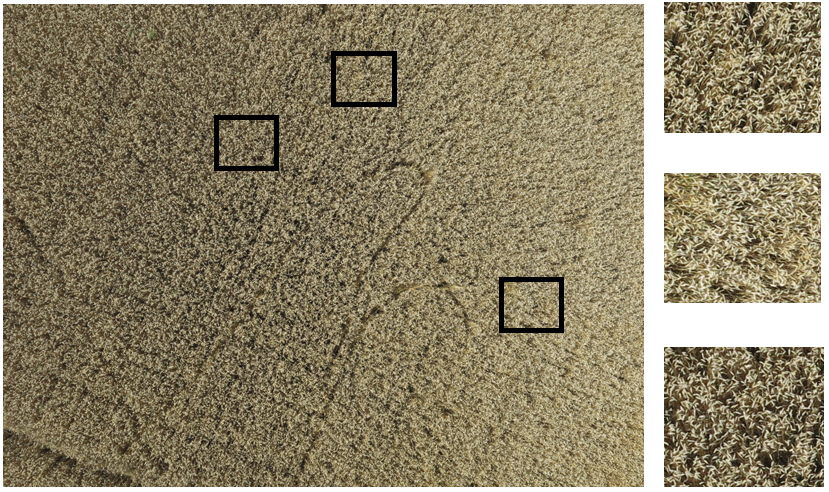
\includegraphics[width=0.85\textwidth]{fig/20a.png}
     %\vspace{-1em}
    \begin{center}    
       \caption{{\footnotesize \textit{Tre tilfældige udsnit taget fra et markbillede.}}}
    \label{fig:korn}
     \end{center}
     \vspace{-2.5em}
  \end{figure} \noindent
Følgende observationer er gjort af markbillederne, samt forhold omkring overflyvningen:
\begin{itemize}
\item{\textbf{Overlap:} Overlappet imellem billederne har en signifikant indflydelse på korrespondanceanalysen. Et stort overlap vil betyde at interessepunkter har større sandsynlighed for at indgå i begge billeder. Derfor, ved mindre overlap, skal der udvælges flere interessepunkter. Det er bekræftet at billederne i gennemsnit overlapper hinanden med ca. 70\%. Overlappet afhænger af hvilken højde billederne er taget på - jo længere fra jorden billedet er taget, jo større er overlappet. Figur \ref{fig:overlap} viser fire billeder, sat sammen parvist, der er taget ved to forskellige højder, hvor billedernes overlap er markeret med blåt. (a) er taget når dronen er på største højde, billederne er estimeret til at overlappe hinanden med ca. 80 $\%$. (b) er taget ved en lavere højde, billederne overlapper hinanden med ca. 35$\%$.
\begin{figure}[H]
    \centering
    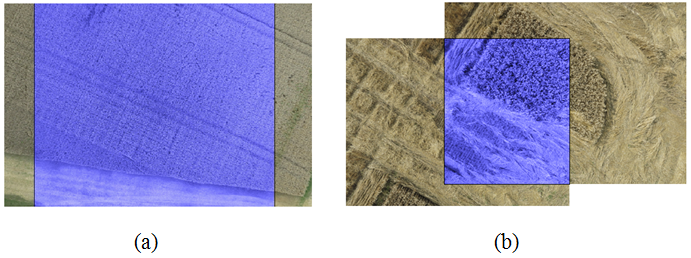
\includegraphics[width=0.85\textwidth]{fig/17.png}
     \vspace{-1em}
    \begin{center}    
       \caption{{\footnotesize \textit{Markbilleder taget ved forskellige højder, det blå område viser billedernes overlap.}}}
    \label{fig:overlap}
     \end{center}
     \vspace{-2.5em}
  \end{figure} \noindent }
\item{\textbf{Rotation:} Der er observeret mindre grad af rotation imellem billederne.
Den største grad af rotation er observeret i de to billeder, hvor dronen er nået kanten og skifter flyveretning. Denne rotation er registreret til at være 10-15$^{\circ}$ og er illustreret i figur \ref{fig:rotation}.
\begin{figure}[H]
    \centering
    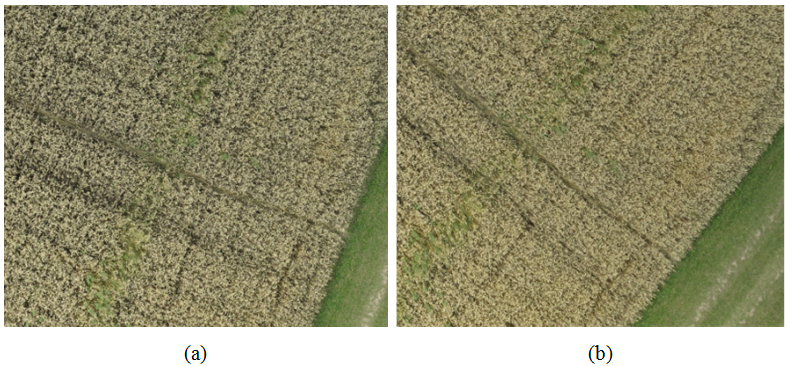
\includegraphics[width=0.85\textwidth]{fig/19.png}
     \vspace{-1em}
    \begin{center} 
       \caption{{\footnotesize \textit{Dronen skal til at ændre flyveretning, hvilket giver rotation imellem billederne.}}}
    \label{fig:rotation}
     \end{center}
     \vspace{-2.5em}
  \end{figure} \noindent}
\item{\textbf{Okklusion:}
I et cirkulært område, hvor kamereet står 90$^{\circ}$ på marken (ca. midten af billedet), vil jorden imellem kornet være mere synligt end i resten af markbilledet.
\begin{figure}[H]
    \centering
    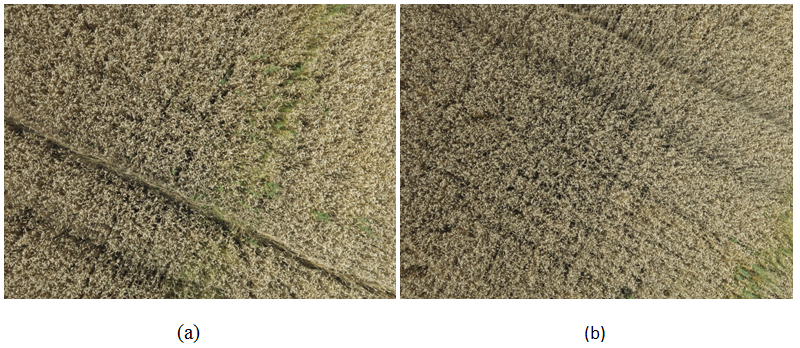
\includegraphics[width=0.85\textwidth]{fig/18.png}
     \vspace{-1em}
    \begin{center}    
       \caption{{\footnotesize \textit{ To forkudte billeder, hvor traktorsporet er okkluderet. }}}
    \label{fig:okklusion}
     \end{center}
     \vspace{-2.5em}
  \end{figure} \noindent
Figur \ref{fig:okklusion} er et eksempel på okklusion af jord, hvor (a) traktor spor optræder direkte under dronen og (b) derefter forskudt. Traktorsporet, der optræder direkte under dronen, er tydelig og man kan se jorden. For det samme traktorspor, i det forskudte billede, er jorden ikke længere synlig.}
%\item{\textbf{Struktur} }
\end{itemize}
\section{Hypoteser}
Ud fra ovenstående analyse er der opstillet følgende hypoteser om krav til de udvalgte metoder:
\begin{itemize}
%\item{ <Det forventes, grundet strukturen af korn, at detektorer som leder efter veldefinerede strukturer, som hjørner, ikke vil have en god effekt på korn, men at blobs vil give bedre resultater.> }
\item{Det forventes ikke at metoderne behøver være invariante overfor rotation, grundet den lille rotation der forekommer imellem billederne. }
\item{Det forventes at metoderne skal være skalainvariante da fotograferingen sker ved skiftende højde.}
\item{ Grundet det til tider lille overlap imellem billederne, forventes det at detektoren skal tilpasses til at finde mange punkter, for at sikre en repeterbar detektion.}
\item{Det forventes ikke at der skal tages højde for problemer ved okklusion. Dog er graden af okklusion større, ved lavere højde, og dette kan have indflydelse på antallet af korrekte korrespondancer.
%Et overvejet tiltag var ikke at undersøge et område direkte under dronen, men det blev konkluderet at .
}
\end{itemize}